\documentclass{beamer}

\usepackage[style=british]{csquotes}
\usepackage[utf8]{inputenc}
\usepackage{amsmath}
\usepackage{xcolor}
\usepackage{hyperref}

%cross over the text
\usepackage{ulem}

\usepackage{graphicx}
\graphicspath{{./images/}}

%bibliography
%\setbeamertemplate{bibliography item}[text] %default is an icon of an article

\title{Deep Learning papers related to MoLAB activities}
\author{Anton Popov}
\institute{UCLM, MoLAB, Spain, Ciudad Real}
%\date{April 16, 2019}

\usetheme{Warsaw}
% insert number of pages to all slides
\newcommand*\oldmacro{}%
\let\oldmacro\insertshorttitle%
\renewcommand*\insertshorttitle{%
	\oldmacro\hfill%
	\insertframenumber\,/\,\inserttotalframenumber}


\begin{document}
	
\begin{frame}
\titlepage
\end{frame}


\begin{frame}
\frametitle{Definitions}
\begin{itemize}
	\item \textbf{Tumor burden(tumor load)} - refers to the number of cancer cells, the size of a tumor, or the amount of cancer in the body.
	
	\item \textbf{Response Evaluation Criteria In Solid Tumor (RECIST)} - A standard way to measure how well a cancer patient responds to treatment. It is based on whether tumors shrink, stay the same, or get bigger. To use Response Evaluation Criteria In Solid Tumors, there must be at least one tumor that can be measured on x-rays, CT scans, or MRI scans. The types of response a patient can have are a complete response (CR), a partial response (PR), progressive disease (PD), and stable disease (SD){\color{gray}(\textit{tumor-centric, not patient centric criteria})}
	
	\item \textbf{Response Assessment in Neuro-Oncology (RANO)} - criteria and requirements for a uniform protocol.
\end{itemize}
\footnote{\url{https://www.cancer.gov/publications/dictionaries}}
\end{frame}



\begin{frame}
\frametitle{RANO paper}
\begin{figure}
	\centering
	
\includegraphics[width=1.0\textwidth]{images/paper_rano_name.png}
\end{figure}
Journal of Clinical Oncology (\href{https://www.ncbi.nlm.nih.gov/pmc/articles/PMC5516482/pdf/JCO.2017.72.7511.pdf}{{\color{blue}\underline{link}}}); June 22, 2017
\end{frame}



\begin{frame}
\frametitle{RANO summary}
\begin{itemize}
	\item multidisciplinary international working group ... working in collaboration with government and industry to \textit{enhance the interpretation of clinical trials related to intracranial tumors}
	\item born out of a workshop conducted by the Jumpstarting Brain Tumor Drug Development Coalition and the US Food and Drug Administration
	\item \textbf{standardized brain tumor imaging protocol now exists to reduce variability and improve reliability}
\end{itemize}

% tell about electrostatic potential - voltage analogy; planes in the sky without clouds
\begin{columns}
	\begin{column}{0.5\textwidth}
\begin{figure}
	\centering
	
\includegraphics[width=0.5\textheight]{images/ruler.jpg}
\end{figure}
	\end{column}
	\begin{column}{0.5\textwidth}
		\textbf{Assumption}: tumors grow in spherical shapes and the 2D measurement of lesion's largest diameter on MRI is a surrogate marker of tumor volume \textit{{\color{gray}(relies on manual two-dimensional measurements...)}}
	\end{column}
\end{columns}
\end{frame}


\begin{frame}
\frametitle{Ways to improve?}
\begin{figure}
	\centering
	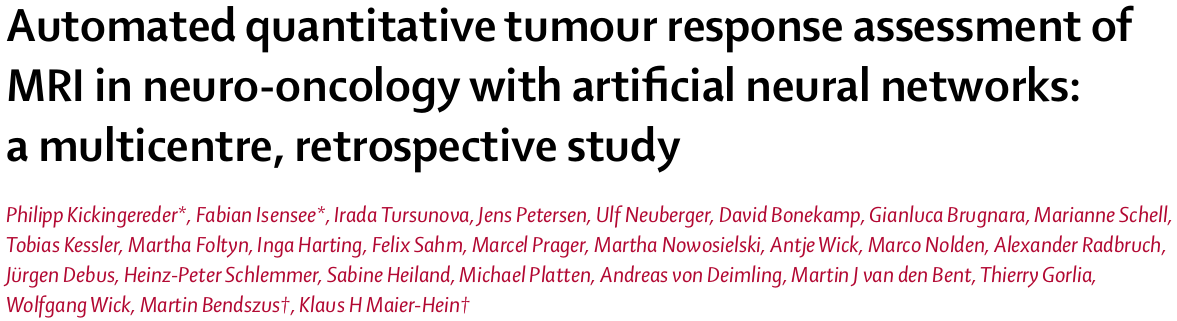
\includegraphics[width=1.0\textwidth]{images/paper_01_name.png}
	\label{fig:full_process}
\end{figure}
Lancet Oncology (\href{https://www.thelancet.com/journals/lanonc/article/PIIS1470-2045(19)30098-1/fulltext}{{\color{blue}\underline{link}}}); April 2, 2019

%https://doi.org/10.1016/S1470-2045(19)30098-1
\end{frame}


\begin{frame}
\frametitle{Definitons and abbreviations in the paper}
\begin{itemize}
	\item \textbf{Definition: }Given two sets $X$ and $Y$:
	$$DICE = \frac{2|X \cap Y|}{|X| + |Y|}$$
	where $|X|$, $|Y|$ - cardinalities of two sets.
	\item $CE$ - contrast-enhancing target lesions
	\item $NE$ - non-enhancing T2-signal abnormalities
\end{itemize}
\end{frame}


%\begin{frame}
%\frametitle{Statistics matters...}
%\begin{figure}
%	\centering
%	\includegraphics[height=0.85\textheight]{images/mcconahi_smokes.jpg}
%\end{figure}
%\end{frame}


\begin{frame}
\frametitle{Results}
Segmentation results:
\begin{itemize}
	\item median DICE on Heidelberg test dataset:
	\begin{itemize}
		\item CE: 0.89 [95\% CI 0.86 - 0.90]
		\item NE: 0.93 [95\% CI 0.92 - 0.94]
	\end{itemize}
	\item median DICE on EORTC-26101 test dataset:
	\begin{itemize}
		\item CE: 0.91 [95\% CI 0.90 - 0.92]
		\item NE: 0.93 [95\% CI 0.93 - 0.94]
	\end{itemize}
\end{itemize}
Hazard ratios:
\begin{itemize}
	\item          ANN: 2.59 [95\% CI 1.86 - 3.60]
	\item central RANO: 2.07 [95\% CI 1.46 - 2.92]; p $<$ 0.0001
\end{itemize}
Yields a 36\% margin over RANO (p $<$ 0.0001) when comparing reliability values(i. e., agreement in the quantitative volumetrically defined time to progression [based on radiologists ground truth $vs$ automated assessment with ANN] of 87\% [266 of 306 with sufficient data] compared with 51\% [155 of 306] with local $vs$ independent central RANO assessment).
\end{frame}


\begin{frame}
\frametitle{Data overview}
\begin{center}
	\begin{tabular}{|c | c | c | c |} 
		\hline
		 & MRI & Patients & Comments \\
		 \hline
		 Train & 455 & 455 & Helidberg training dataset \\
		 \hline
		 Test & 239 & 40 & Heildelberg testing dataset \\
		  & 2034 & 532 & EORTC-26101 study (\href{https://clinicaltrials.gov/ct2/show/NCT01290939}{\color{blue}\underline{link}}) \\
		  \hline
		  Simulate & 595 & 466 & Heildelberg simulation dataset \\
		  \hline
	\end{tabular}
\end{center}

All Heildelberg datasets includes:
\begin{itemize}
	\item T1-weighted (before contrast agent)
	\item cT1-weighted (after contrast agent)
	\item fluid-attenuated inversion recovery (FLAIR)
	\item T2-weighted images
\end{itemize}
IMHO feeding all modalities makes sense (\href{https://openreview.net/pdf?id=Bygh9j09KX}{{\color{blue}\underline{link}}}).
\end{frame}


\begin{frame}
\frametitle{Helidberg training dataset}
\begin{center}
	\begin{tabular}{ p{7.0cm} | p{3.5cm} } 
		\hline
		Feature & Comment\\ [0.5ex]
		\hline\hline
		"histologically confirmed glioblastoma or lower-grade glioma (including diffuse astrocytic and oligodendroglial WHO grade II and III tumours)" & GB and LGG looks differently $\rightarrow$ expressive ANN is needed\\
		\hline
		"single timepoint: preoperatively from initial diagnosis or early postoperatively ... or at follow-up and was specifically ensembled to represent the broad phenotypic appearence of brain tumours on MRI during disease evolution" & preoperatively, postoperatively, follow-up mixed  together $\rightarrow$ expressive ANN is needed\\
		\hline
		appropriate MRI scans were manually identified to enrich the dataset with comparatively uncommon and difficult cases on the basis of the judgement of the neuroradiologists & only patients with disease\\
		\hline
		\hline
	\end{tabular}
\end{center}
\end{frame}


\begin{frame}
\frametitle{Helidberg Test / Simulate datasets}
Excellent example of following \href{https://developers.google.com/machine-learning/guides/rules-of-ml/}{{\color{blue}\underline{recommendations}}} from Google (Rule 5: Test the infrastructure independently from the ML).
\vskip 1cm
\begin{columns}
	\begin{column}{0.5\textwidth}
		\centering
		\textbf{Test} \\
		This dataset was a longtitudinal dataset with preoperative and consequtive follow-up scans
	\end{column}
	\begin{column}{0.5\textwidth}
		\centering
		\textbf{Simulate} \\
		Cohort of adult patients for testing of the developed infrastructure for automated tumour segmentation and quantitative assessment of tumour response in a simulated clinical environment
	\end{column}
\end{columns}
\end{frame}


\begin{frame}
\frametitle{Process}
\begin{figure}
	\centering
	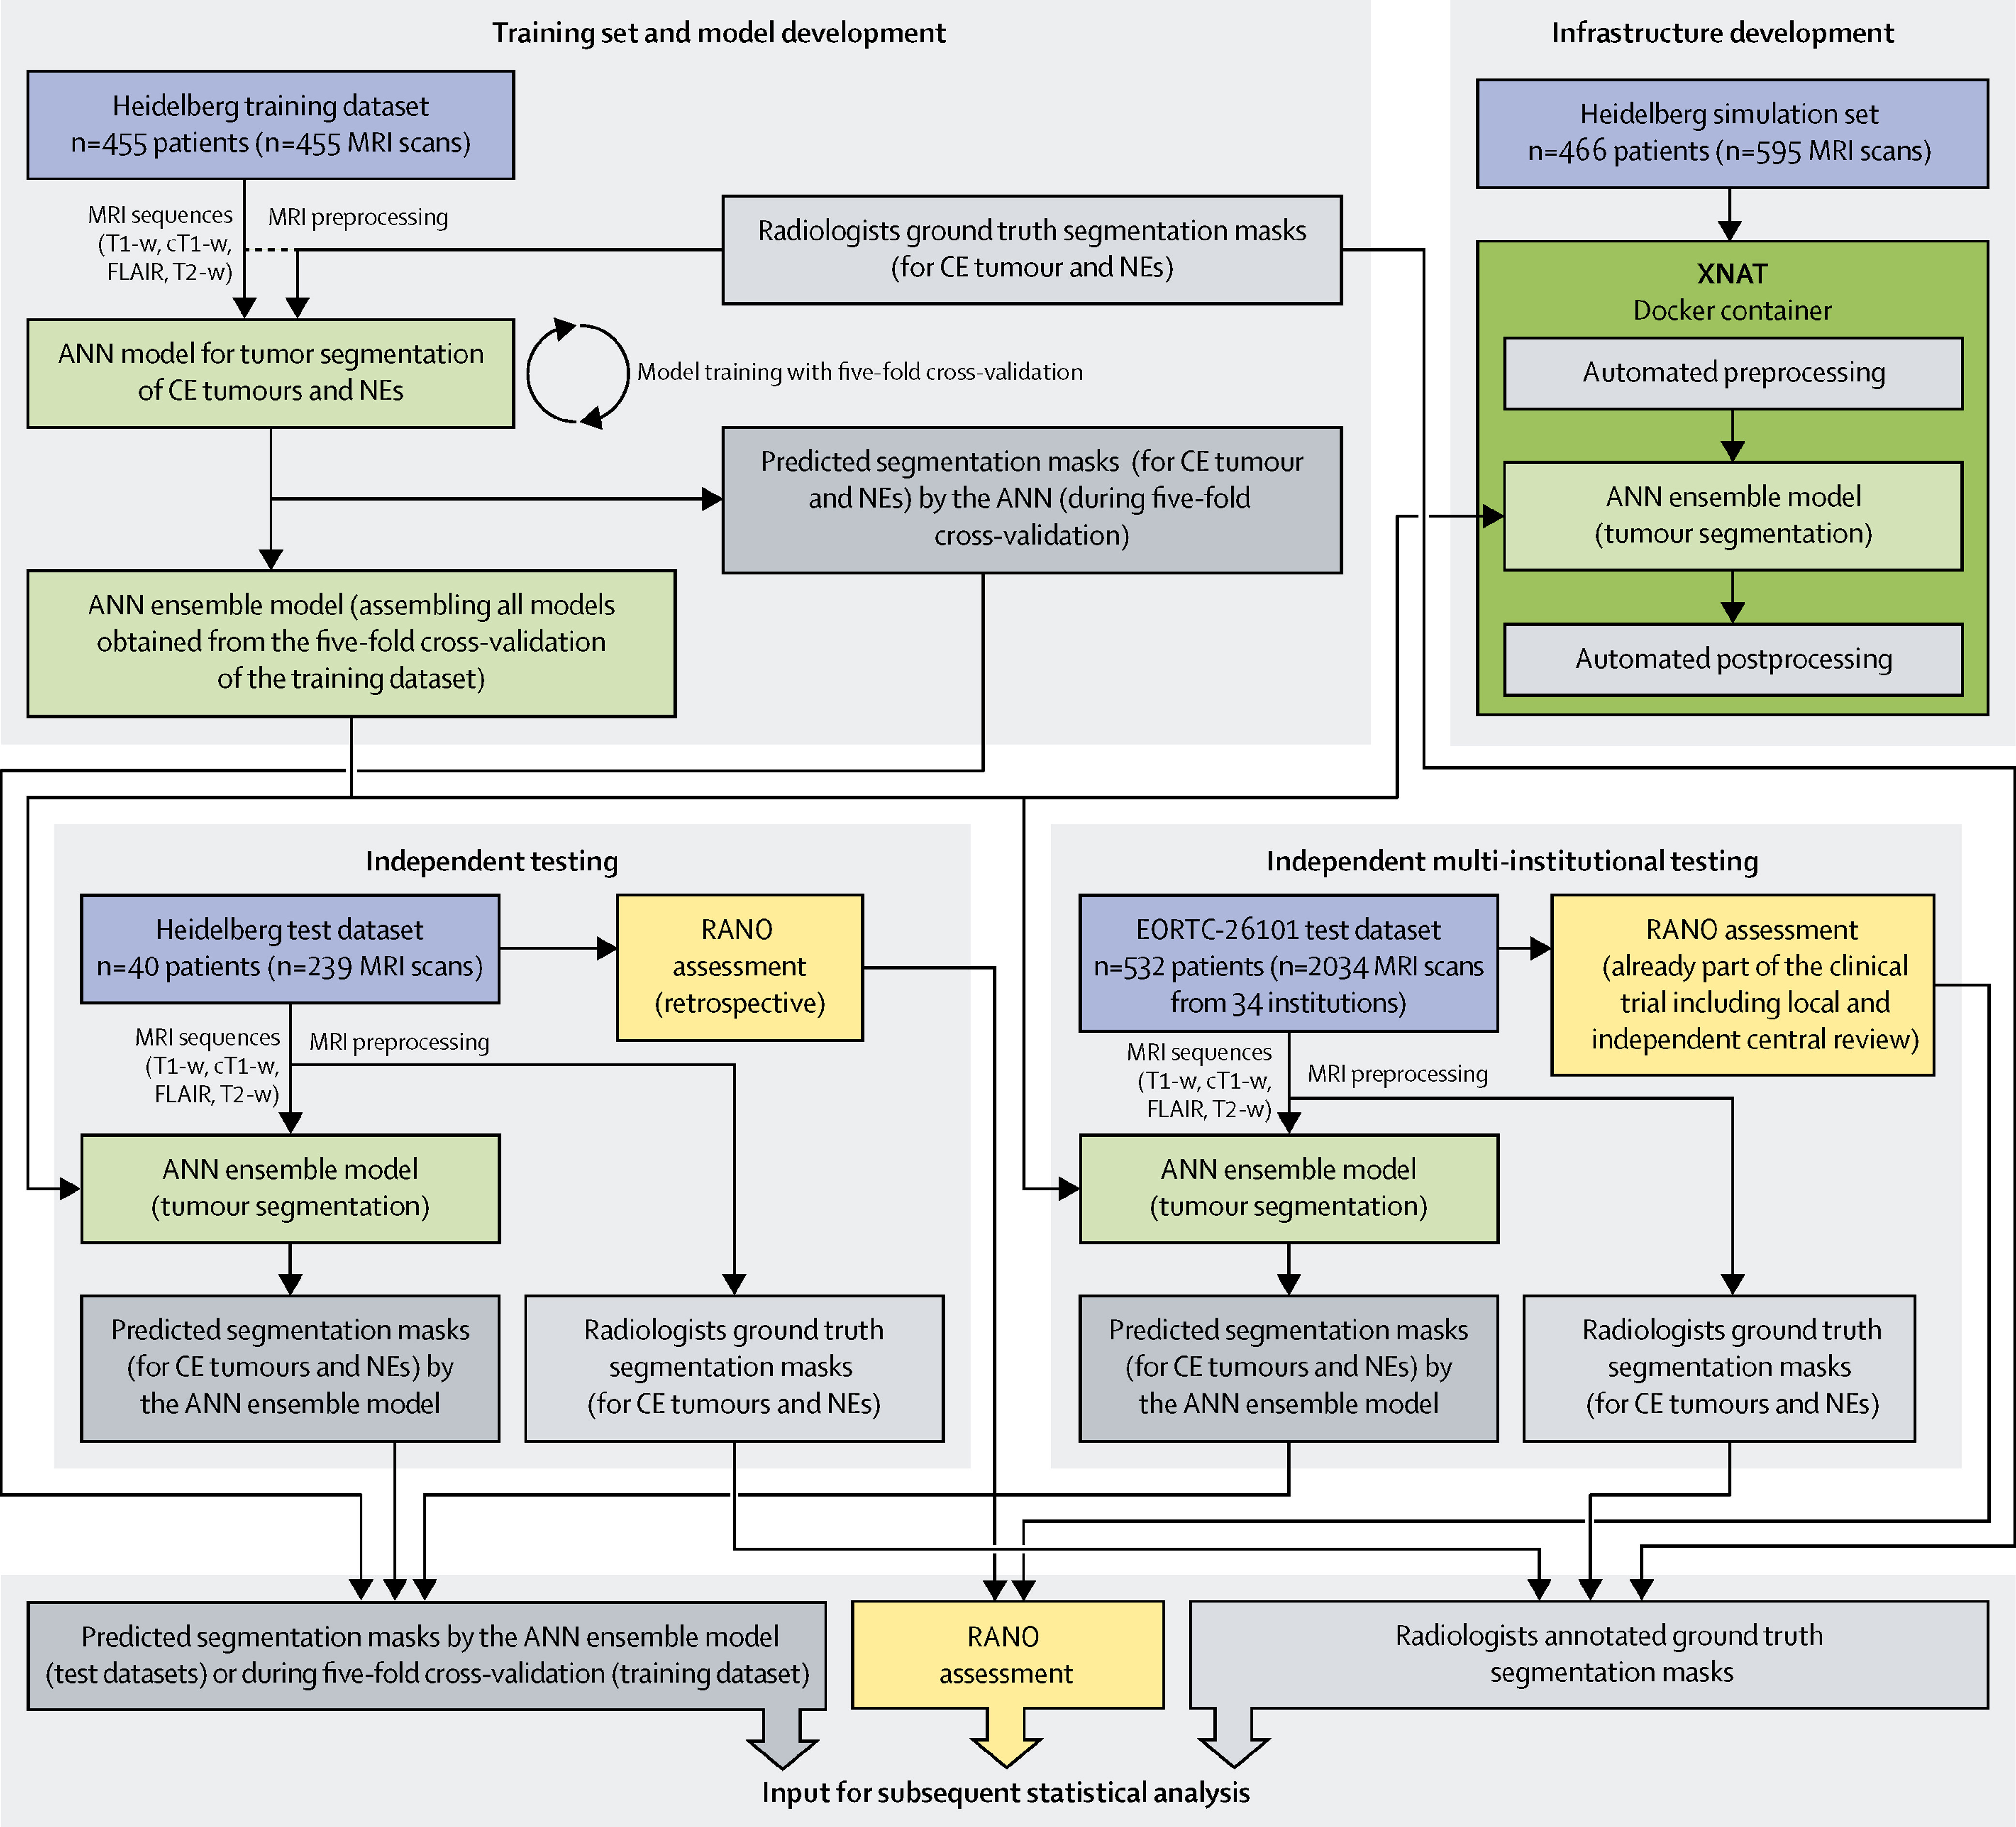
\includegraphics[height=.9\textheight]{images/im_process.jpg}
\end{figure}
\end{frame}


\begin{frame}
\frametitle{Infrastructure}
\begin{figure}
	\centering
	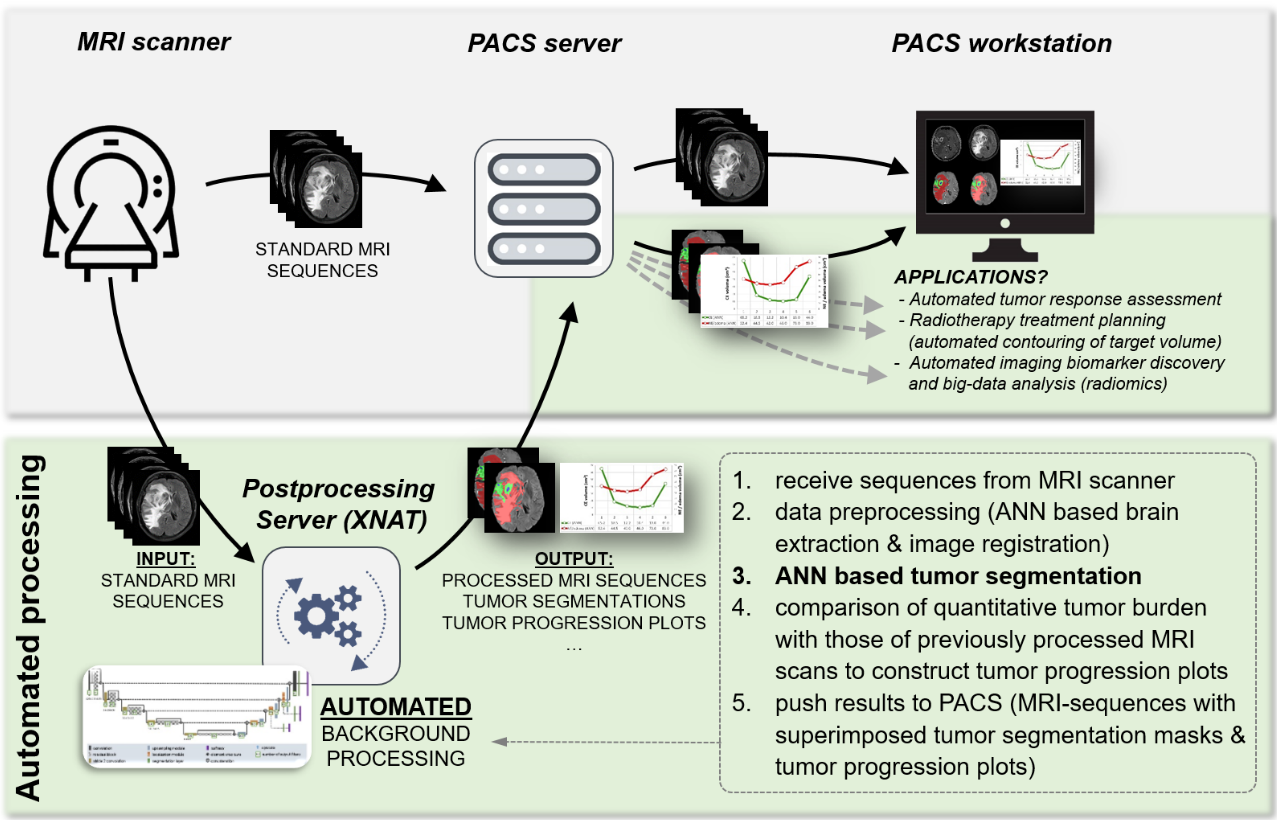
\includegraphics[width=1.2\textheight]{images/paper_1_infrastructure.png}
\end{figure}
%\textit{PACS} - picture archiving and communication system
\end{frame}


\begin{frame}
\frametitle{Architecture from Elies Fuster presentation}
%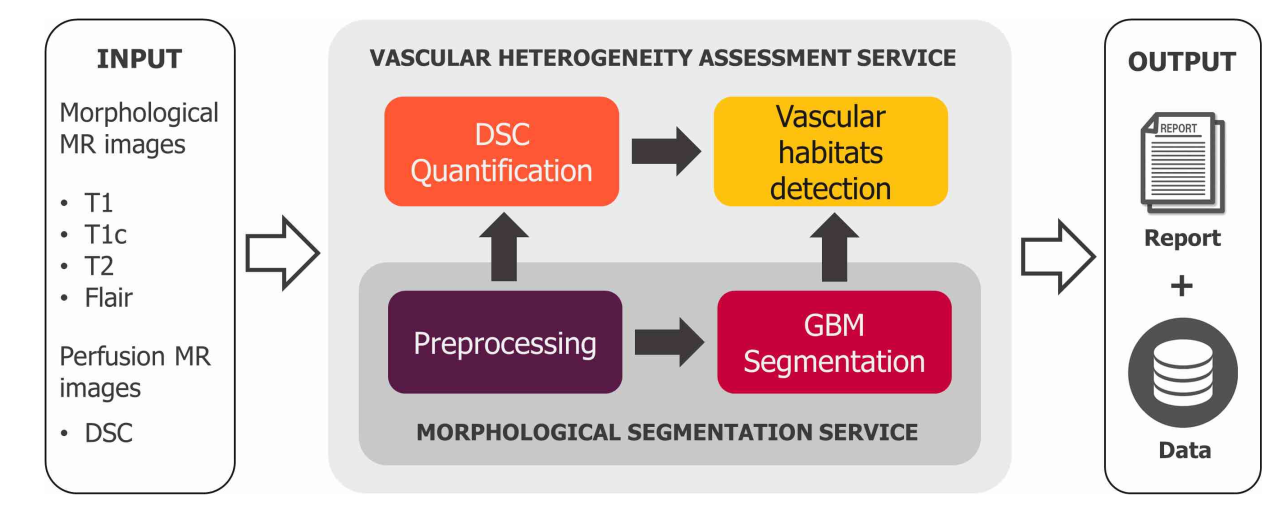
\includegraphics[width=\textwidth]{images/elies_1.png}
\begin{columns}
	\begin{column}{0.5\textwidth}
		\begin{figure}
			\centering
			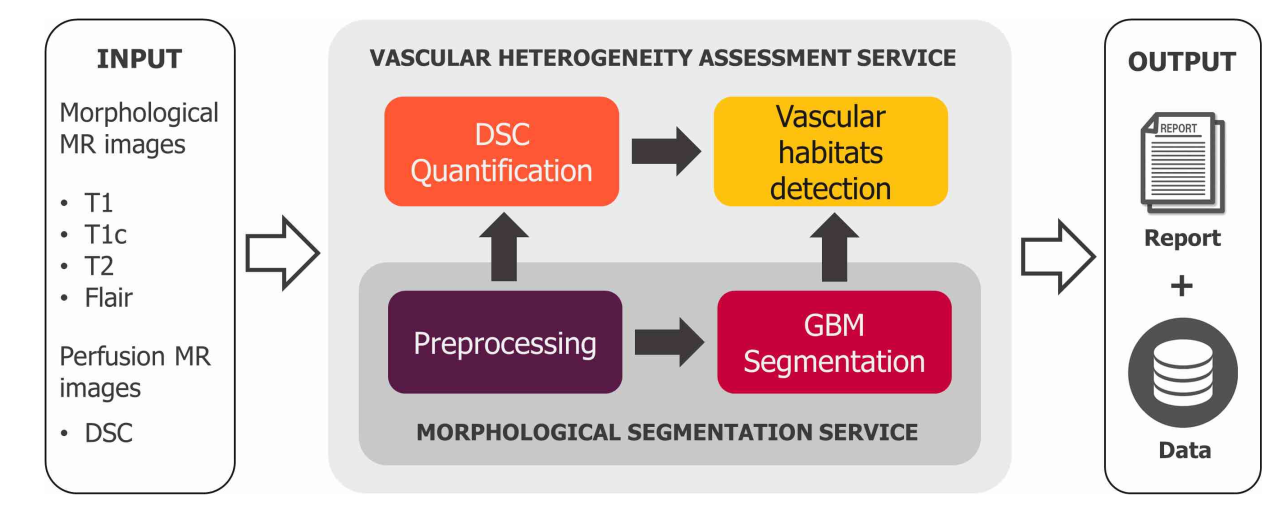
\includegraphics[width=\textwidth]{images/elies_1.png}
			\caption{MRI $\rightarrow$ processing $\rightarrow$ output}
		\end{figure}
	\end{column}
	\begin{column}{0.5\textwidth}
		\begin{figure}
			\centering
			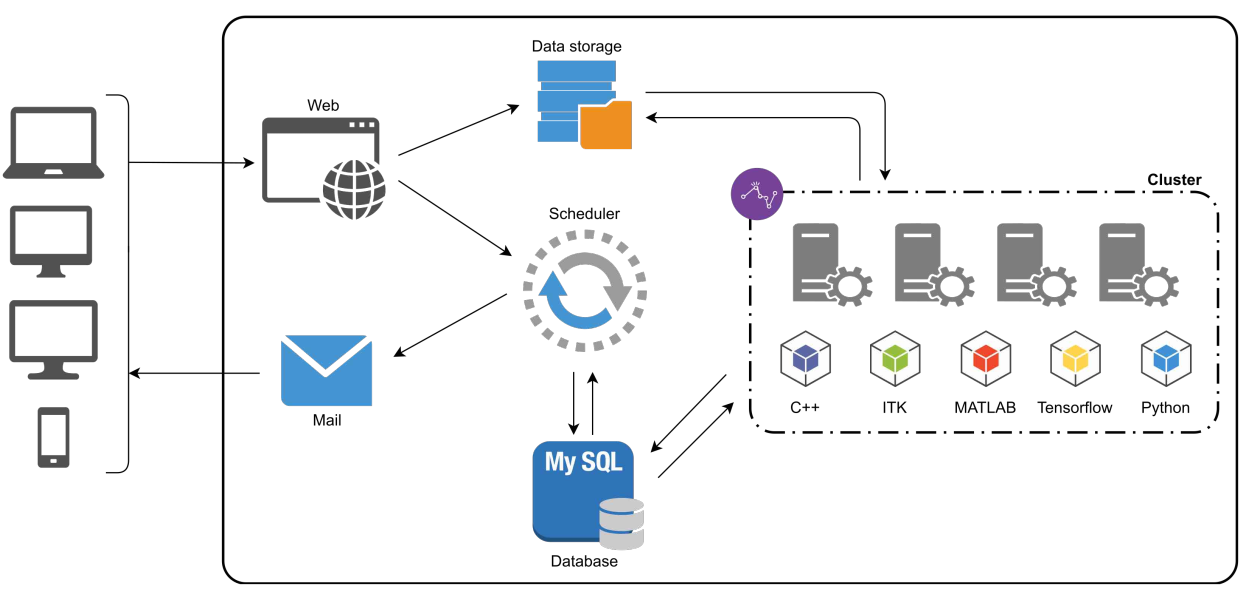
\includegraphics[width=\textwidth]{images/elies_2.png}
			\caption{Standard Web-app}
		\end{figure}
	\end{column}
\end{columns}
Notes:
\begin{itemize}
	\item the system is functioning
	\item separate storage of MRI images and other data
\end{itemize}
\end{frame}


\begin{frame}
\frametitle{Proof of concept - Classification Web App}
\begin{columns}
	\begin{column}{0.55\textwidth}
		\begin{figure}
			\centering
			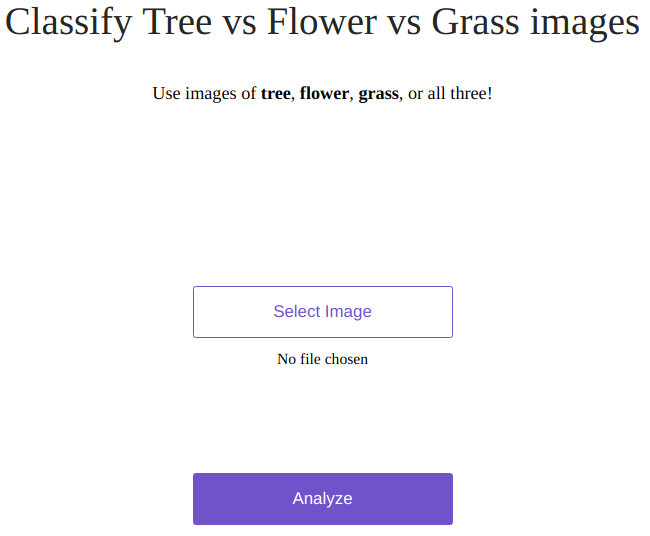
\includegraphics[width=1.0\textwidth]{images/render_classifier.png}
		\end{figure}
	\end{column}
	\begin{column}{0.45\textwidth}
		This app (\href{https://tree-grass-flower.onrender.com/}{{\color{blue}\underline{tree-grass-flower.onrender.com}}}) is running on render.com platform. After image uploading user receives class prediction.
	\end{column}
\end{columns}
\end{frame}


\begin{frame}
\frametitle{Training set and model development}
\begin{figure}
	\centering
	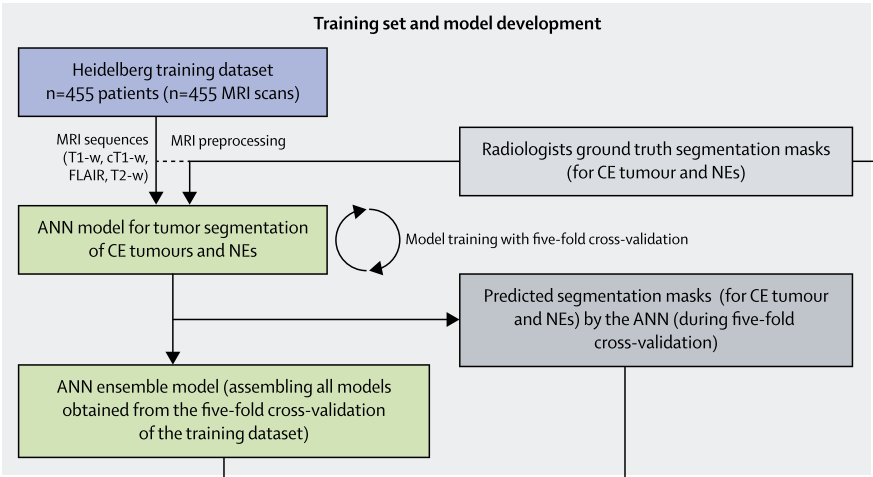
\includegraphics[width=\textwidth]{images/process_training.png}
\end{figure}
\end{frame}


\begin{frame}
\frametitle{Neural Network architecture}
\begin{figure}
	\centering
	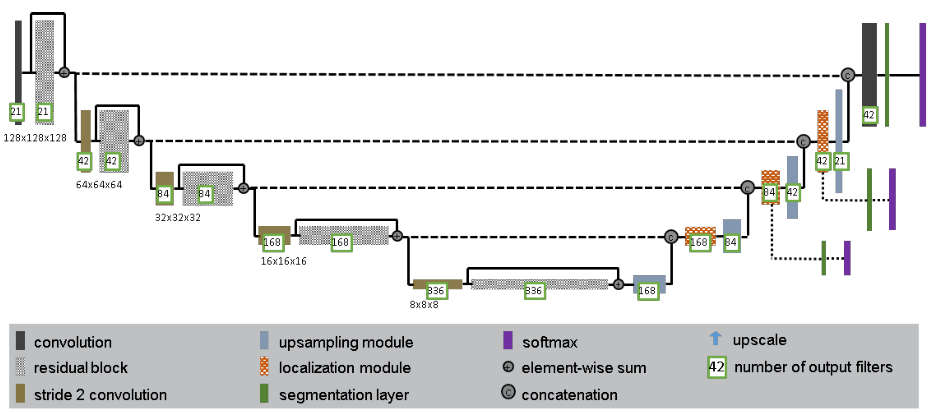
\includegraphics[width=\textwidth]{images/paper_1_architecture.png}
\end{figure}
Inspired by \href{https://arxiv.org/abs/1505.04597}{{\color{blue}\underline{U-Net}}} and utilizes \href{https://arxiv.org/abs/1512.03385}{{\color{blue}\underline{residual blocks}}} in encoder.
\end{frame}


\begin{frame}
\frametitle{ResNet}
\begin{columns}
	\begin{column}{0.5\textwidth}
		\begin{figure}
			\centering
			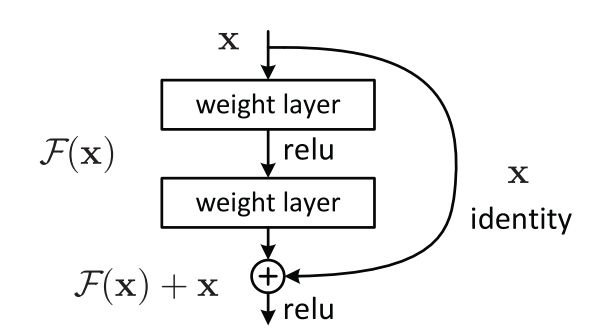
\includegraphics[width=\textwidth]{images/resnet_block.png}
		\end{figure}
	\begin{itemize}
		\item ResNet introduce \textbf{skip connection}
		\item solves \textit{vanishing(exploding) gradient} problem
	\end{itemize}
	\end{column}
	\begin{column}{0.5\textwidth}
		\centering
		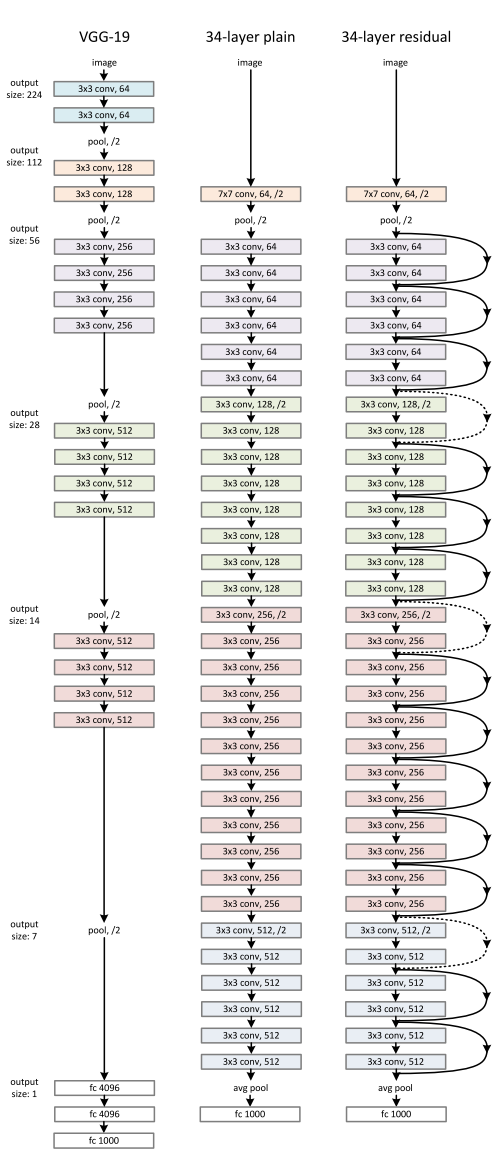
\includegraphics[height=0.85\textheight]{images/resnet_imagenet.png}
	\end{column}
\end{columns}
\end{frame}


\begin{frame}
\frametitle{General notes about the paper}
\begin{itemize}
	\item Appendix contains more technical/useful information
	\item Links to software/technologies that were used are provided (e. g. \href{https://www.xnat.org/}{{\color{blue}\underline{www.xnat.org}}})
	\item Infrastructure notes:
		\begin{itemize}
			\item \href{https://www.docker.com/}{{\color{blue}\underline{Docker}}} container utilization, \href{https://github.com/docker/swarm}{{\color{blue}\underline{Docker Swarm}}} parallelization
			\item open-source only components
			\item code is available on  \href{https://github.com/MIC-DKFZ/HD-BET}{{\color{blue}\underline{GitHub}}}
		\end{itemize}
	\item Network architecture
	\begin{itemize}
		\item Heavy encoder, light decoder
		\item Large Input Patch Size (128 $\times$ 128 $\times$ 128 voxels)
		\item Auxiliary Loss Layers (autograd understanding)
		\item Nonlinearity and Normalization
		\begin{itemize}
			\item instance normalization
			\item leaky ReLU activation function
		\end{itemize}
	\end{itemize}
\end{itemize}
\end{frame}


\begin{frame}
\frametitle{Paper from Gabriel}
\begin{figure}
	\centering
	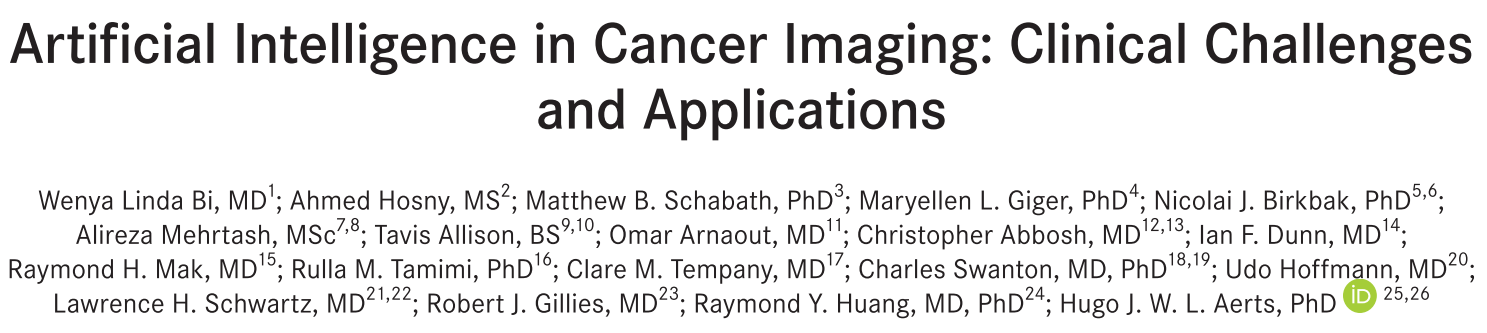
\includegraphics[width=1.05\textwidth]{images/paper_02_name.png}
	\label{fig:full_process}
\end{figure}
CA: a cancer journal for clinicians (\href{https://onlinelibrary.wiley.com/doi/full/10.3322/caac.21552}{\color{blue}{\underline{link}}}); February 5, 2019


Overview for medical doctors. Covers works over lung, brain, breast and prostate cancers at detection, characterization and monitoring of tumors tasks with next key points:
\begin{itemize}
	\item aggregation of multiple data streams(e.g. "imaging genomics")
	\item importance of early diagnosing
	\item AI has the potential to increase efficiency, reproducibility but still in its infancy
\end{itemize}
\end{frame}


\begin{frame}
\frametitle{One of the four best paper of the NeuralIPS}
\begin{figure}
	\centering
	
\includegraphics[width=\textwidth]{images/neural_ordinary_differential_equations.png}
\end{figure}
NeuralIPS, 2018 (\href{https://arxiv.org/abs/1806.07366}{{\color{blue}\underline{link}}})


YouTube explanation from Siraj Raval is \href{https://www.youtube.com/watch?v=AD3K8j12EIE}{{\color{blue}\underline{here}}}.
\end{frame}


\begin{frame}
\frametitle{Geometric deep learning}
\begin{figure}
	\centering
	
\includegraphics[width=\textwidth]{images/geometric_deep_learning.png}
\end{figure}
IEEE Signal Processing Magazine, 2016 (\href{https://arxiv.org/abs/1611.08097}{{\color{blue}\underline{link}}})
\end{frame}


\begin{frame}
\frametitle{Neural networks interpretation}
\begin{figure}
	\centering
	
\includegraphics[width=0.8\textwidth]{images/interpretation_nn.png}
\end{figure}
Analytical Chemistry Research, 2014 (\href{https://cs.nyu.edu/~fergus/papers/zeilerECCV2014.pdf}{{\color{blue}\underline{link}}})
\end{frame}


\begin{frame}
\frametitle{Adversarial attacks}
\begin{figure}
	\centering
	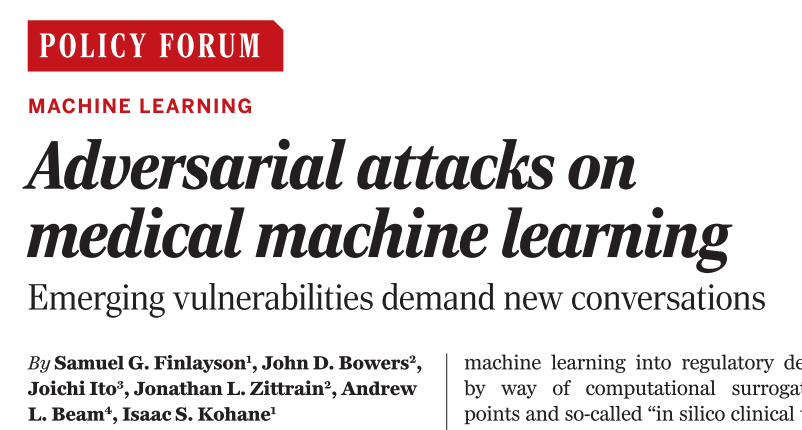
\includegraphics[width=\textwidth]{images/adversarial.png}
\end{figure}
Science, March 22, 2019
(\href{https://science.sciencemag.org/content/363/6433/1287}{{\color{blue}\underline{link}}})
\vfill
\href{https://www.technologyreview.com/s/613555/how-we-might-protect-ourselves-from-malicious-ai/}{{\color{blue}\underline{MIT Technology Review}}} article
\end{frame}


\begin{frame}
\frametitle{Breast cancer risk predictions}
\begin{columns}
	\begin{column}{0.5\textwidth}
		\begin{figure}
			\centering
			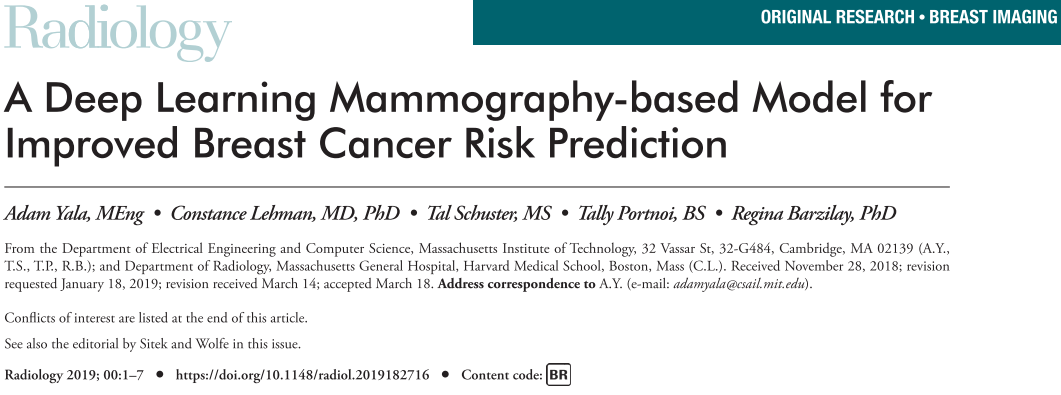
\includegraphics[width=\textwidth]{images/breast_cancer_5_years.png}
		\end{figure}
	\end{column}
	\begin{column}{0.5\textwidth}
		\begin{figure}
			\centering
			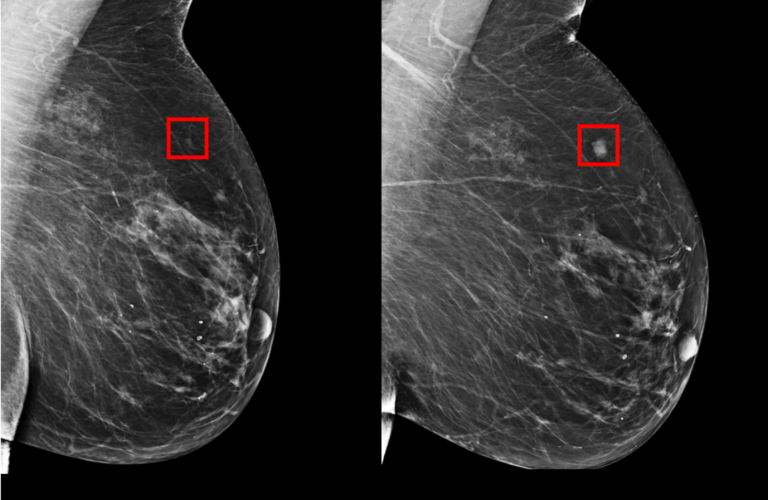
\includegraphics[width=\textwidth]{images/BreastCancerAI.png}
		\end{figure}
	\end{column}
\end{columns}
Radiology, May 7, 2019 (\href{https://pubs.rsna.org/doi/10.1148/radiol.2019182716}{{\color{blue}\underline{link}}})
\begin{itemize}
	\item predicts breast cancer in 4 years before it actually occurs
\end{itemize}
\end{frame}


\begin{frame}
\frametitle{End-to-end lung cancer screening}
\begin{figure}
	\centering
	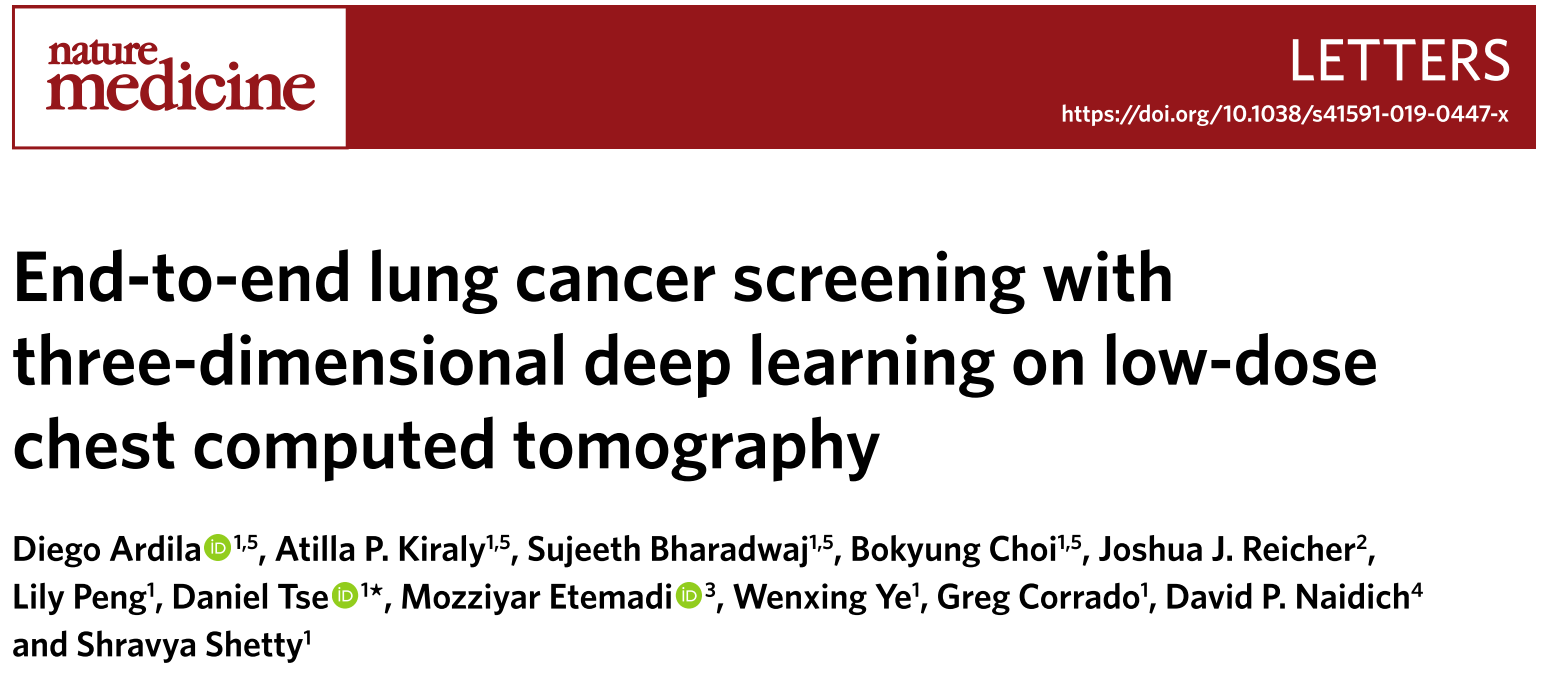
\includegraphics[width=\textwidth]{images/lung_cancer_end.png}
\end{figure}
Nature Medicine, May 20, 2019 (\href{https://www.nature.com/articles/s41591-019-0447-x}{{\color{blue}\underline{link}}})
\begin{itemize}
	\item outperforms ensemble of experienced radiologists
\end{itemize}
\end{frame}


\begin{frame}
\frametitle{Deep Learning is hard... tribute to Fast.AI}
\begin{columns}
	\column{0.8\textwidth}
	\begin{figure}
		\centering
		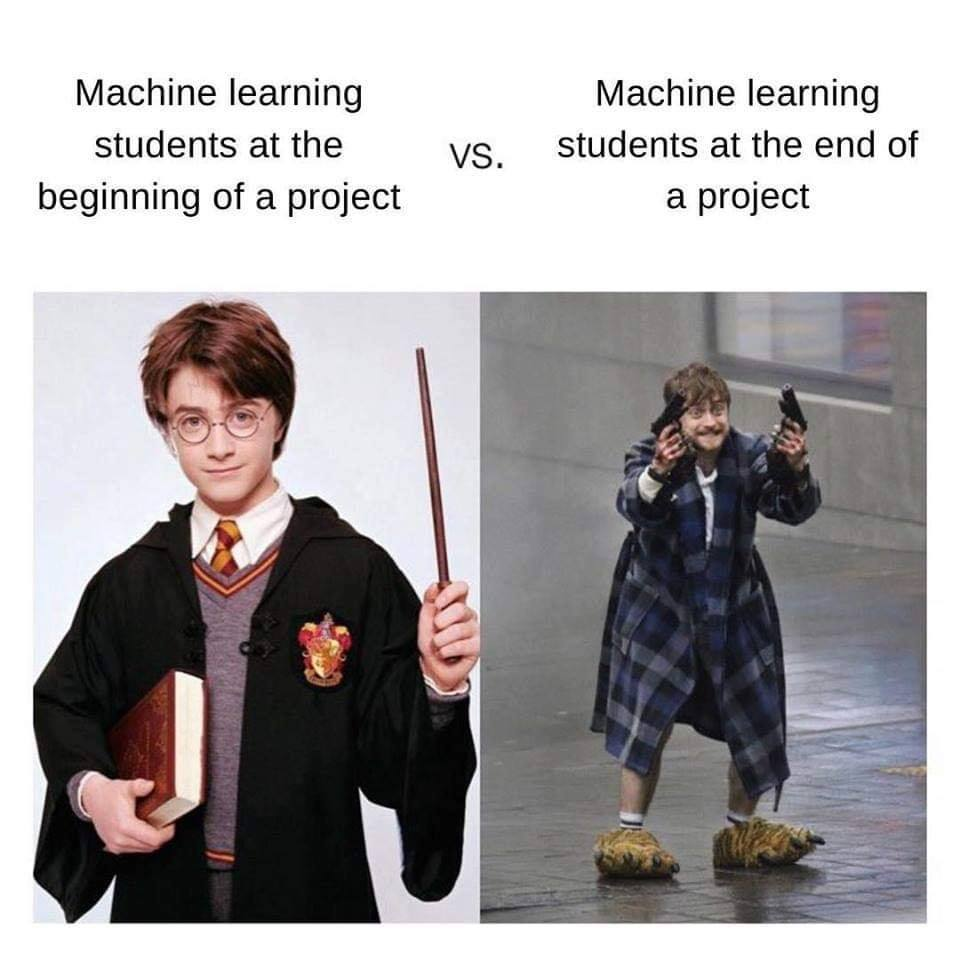
\includegraphics[height=0.9\textheight]{images/harry_ml.jpg}
	\end{figure}
	\column{0.2\textwidth}
	%\textbf{fastai} library was developed to democratize Deep Learning and to reduce number of such transformations of \sout{Gryffindor}ML-students.
	\textbf{Understand something is}:
	\begin{enumerate}
		\item learn how to use it
		\item become familiar with it
	\end{enumerate}
\end{columns}
\end{frame}


\begin{frame}
\frametitle{Example of Fast.AI library usage}
\begin{columns}
	\begin{column}{0.6\textwidth}
		\centering
		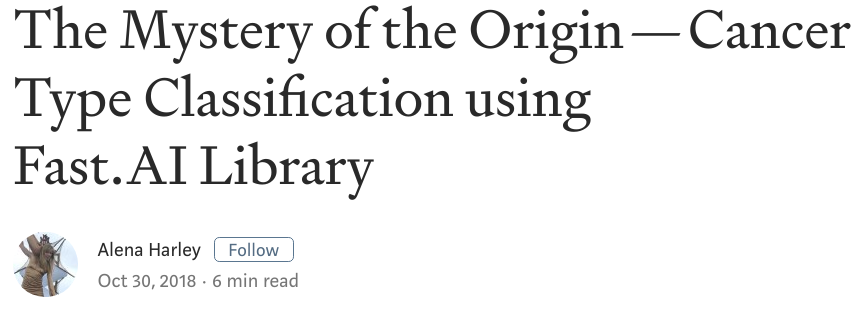
\includegraphics[width=\textwidth]{images/harley_1.png}
	\end{column}
	\begin{column}{0.4\textwidth}
		\centering
		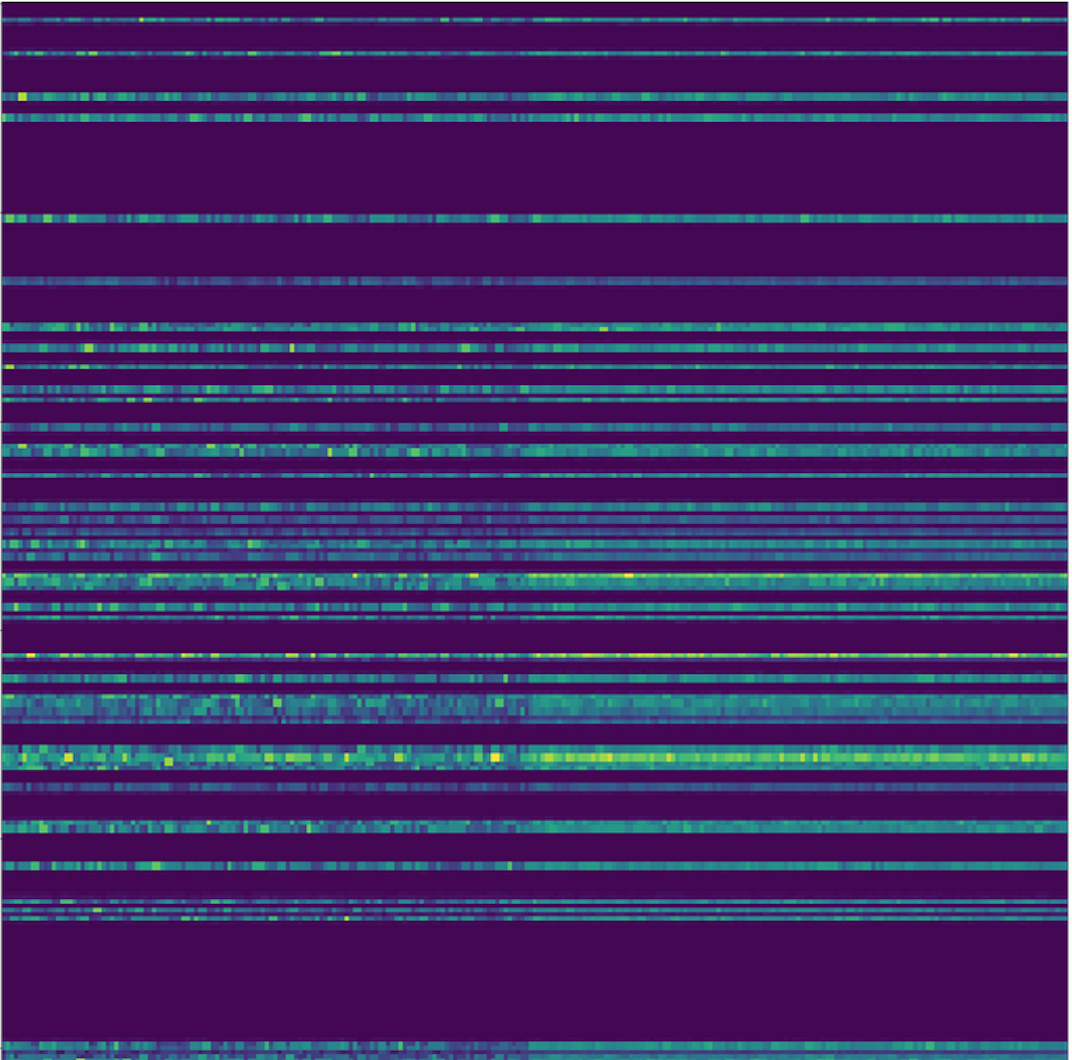
\includegraphics[width=\textwidth]{images/harley_2.png}
	\end{column}
\end{columns}
\vfill
Alena Harley, October 30, 2018 (\href{https://towardsdatascience.com/the-mystery-of-the-origin-cancer-type-classification-using-fast-ai-libray-212eaf8d3f4e}{{\color{blue}\underline{towardsdatascience.com}}})
\end{frame}


\begin{frame}
\frametitle{Meningioma dataset}
\begin{figure}
	\centering
	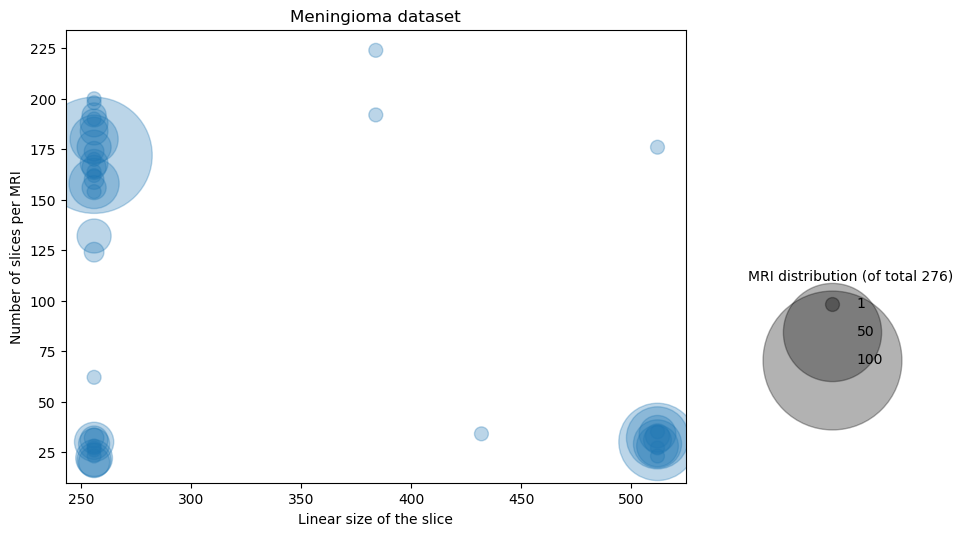
\includegraphics[width=1.0\textwidth]{images/meningioma_dataset.png}
\end{figure}
\end{frame}



\begin{frame}
\frametitle{Brain metastasis dataset}
\begin{figure}
	\centering
	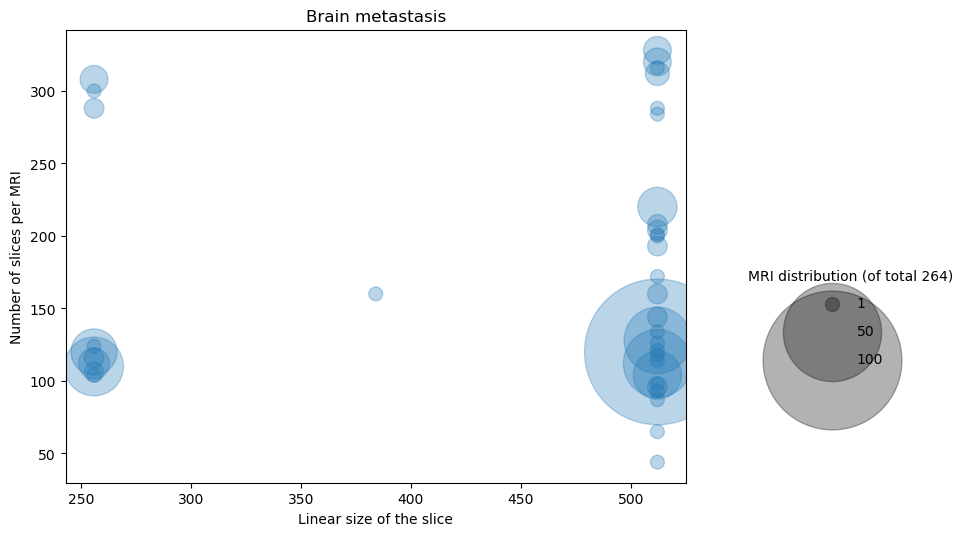
\includegraphics[width=1.0\textwidth]{images/brain_metastasis_dataset.png}
\end{figure}
\end{frame}


\begin{frame}
\frametitle{High grade glioma dataset}
\begin{figure}
	\centering
	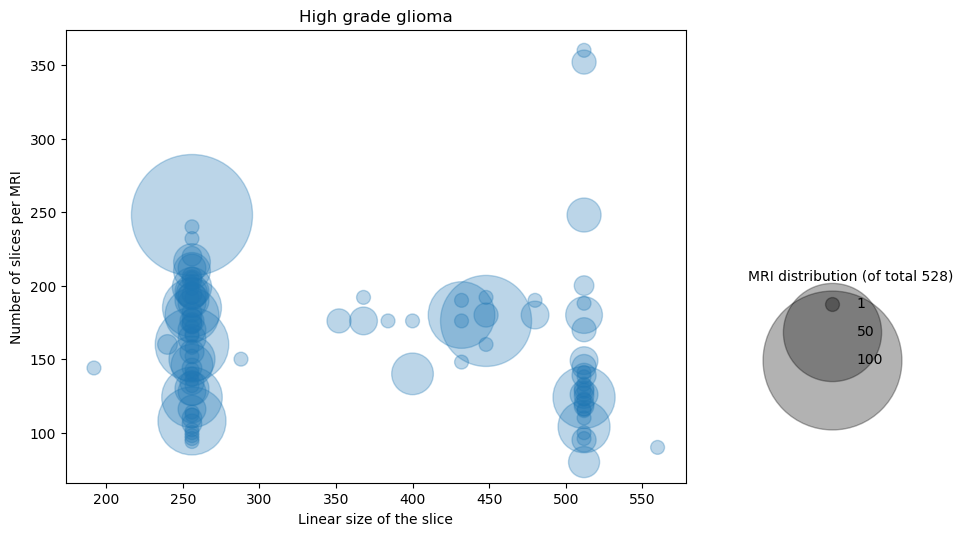
\includegraphics[width=1.0\textwidth]{images/high_grade_glioma_dataset.png}
\end{figure}
\end{frame}


\begin{frame}
\frametitle{Classification data splitting}
\begin{columns}
	\begin{column}{0.5\textwidth}
		Number of non-empty slices:
		\begin{itemize}
			\item Gliomat - 16594
			\item Meningioma - 7607
			\item Metastasis - 5806
		\end{itemize}
	\end{column}
	\begin{column}{0.5\textwidth}
		Dataset splitting:
		\begin{itemize}
			\item Train - 70\%
			\item Validate - 20\%
			\item Test - 10\%
		\end{itemize}
		Data was splitted by patient, i.e. slices from the same MRI can not be in more than one subgroup. 
	\end{column}
\end{columns}
\vspace{1cm}
\centering
Images were resized to 224 $\times$ 224\\
ANN architecture - ResNet34.
\end{frame}


\begin{frame}
\frametitle{Confusion matrix on validation data}
\begin{columns}
	\begin{column}{0.45\textwidth}
		Training losses
		\begin{figure}
			\centering
			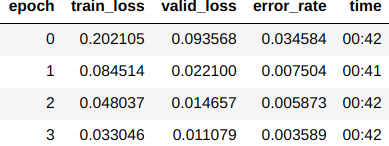
\includegraphics[width=1.0\textwidth]{images/classification_loss_1.png}
		\end{figure}
		Fine-tuning losses
		\begin{figure}
			\centering
			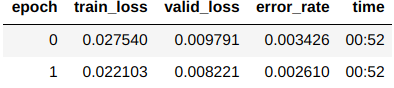
\includegraphics[width=1.0\textwidth]{images/classification_loss_2.png}
		\end{figure}
	\end{column}
	\begin{column}{0.55\textwidth}
%		Confusion matrix
		\begin{figure}
			\centering
			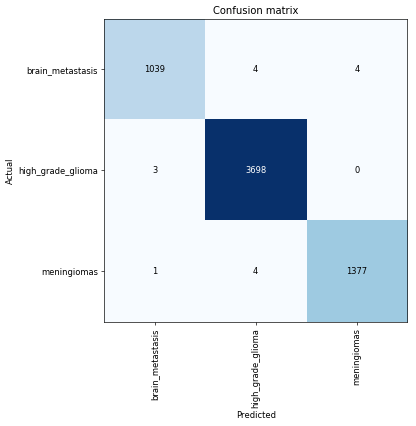
\includegraphics[width=1.0\textwidth]{images/classification_confusion_matrix.png}
		\end{figure}
	\end{column}
\end{columns}
\textit{Validation data is used during the training process for classifier quality evaluation. Confusion matrix above shows how ANN approximated train dataset with respect to validation dataset criterion.}
\end{frame}


\begin{frame}
\frametitle{Confusion matrices on the unseen test data}
\begin{columns}
	\begin{column}{0.5\textwidth}
		\begin{figure}
			\centering
			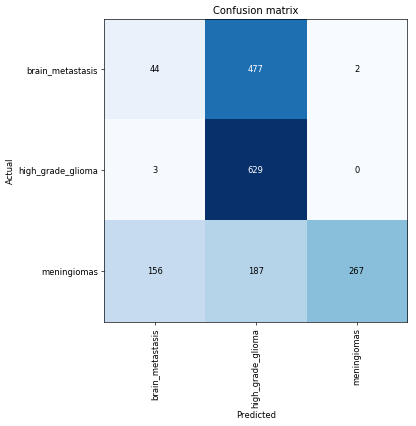
\includegraphics[width=\textwidth]{images/confusion_1.png}
		\end{figure}
	\end{column}
	\begin{column}{0.5\textwidth}
		\centering
		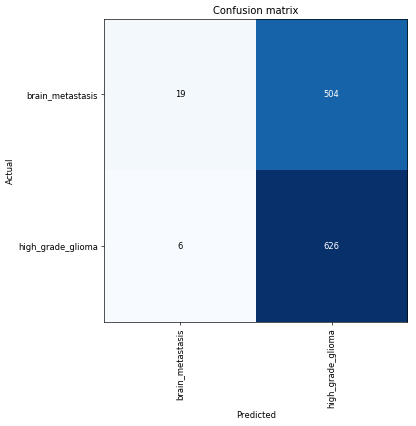
\includegraphics[width=\textwidth]{images/confusion_2.png}
	\end{column}
\end{columns}
\textit{So we see that classifier does not work. Meningioma is distributed over all classes. Brain metastasis are put in the HGG class.}
\end{frame}


\begin{frame}
\frametitle{Ideas for improvement}
\begin{itemize}
	\item Super-resolution like pre-processing;
	\item Generative Adversarial Networks \href{https://news.developer.nvidia.com/ai-can-generate-synthetic-mris-to-advance-medical-research/}{{\color{blue}\underline{generated datasets}}};
	\item "Dumb" 3D synthetic dataset formed with ellipsoids, MRI structure and noise (Gaussian, Rice etc.). Probably I will run it on \href{https://colab.research.google.com/}{{\color{blue}{\underline{Google Colab}}}} platform
	\item Use  Google's \href{https://ai.googleblog.com/2019/05/announcing-open-images-v5-and-iccv-2019.html}{{\color{blue}\underline{Open Images V5}}} dataset for 2D segmentation pretration.
	\item Use federated learning - centralized model with decentralized data (details are in Google comics \href{https://federated.withgoogle.com/}{{\color{blue}\underline{here}}})
\end{itemize}
\end{frame}


\begin{frame}
\frametitle{Competitions}
\begin{columns}
	\begin{column}{0.5\textwidth}
		\centering
		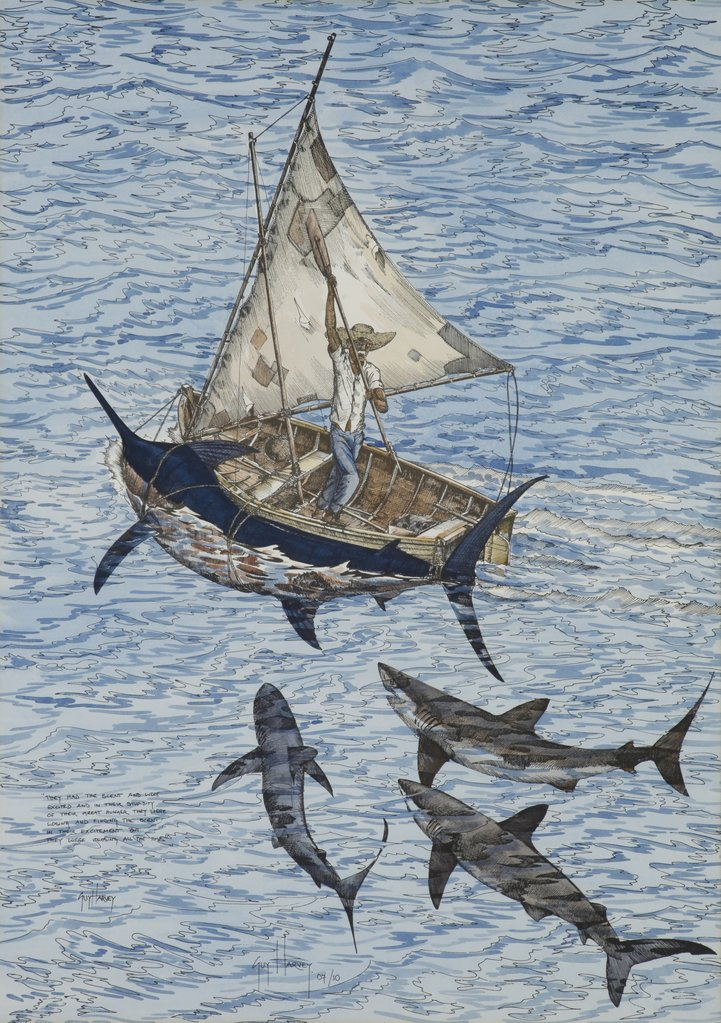
\includegraphics[width=1.0\textwidth]{images/old_man_and_the_sea_3.jpg}
	\end{column}
	\begin{column}{0.5\textwidth}
		%\centering
		Current competitions:
		\begin{itemize}
			\item PAIP2019
			\item ...
		\end{itemize}
		Aim is to reach TOP 10\%. People there usually know what are they doing.
		More medical related ML competition can be found \href{https://grand-challenge.org/challenges/}{{\color{blue}\underline{here}}}.
	\end{column}
\end{columns}
\end{frame}


\begin{frame}
\frametitle{Questions}
\centering
\Huge{¡Gracias!}
\begin{figure}
	\centering
	
\includegraphics[width=0.5\textwidth]{images/qrcode.png}
\end{figure}
\end{frame}


\end{document}
